\chapter{Results}
%Looking also at the general picture usually helps, for example, looking at figure \ref{heatmap}, it is clear that way more paths ended up hitting the lights on the ceiling and on the staircase rather than the two light portals down the hall

Assessing the validity of a tool without performing user tests is often pointless but, due to the complexity of the tool, there was no time to perform any. In their absence, the analysis of two couples of significant datasets are presented.

\section{Couple \#1}

\section{Couple \#2}

\begin{figure}
	\centering
	\begin{subfigure}[t]{0.32\linewidth}
		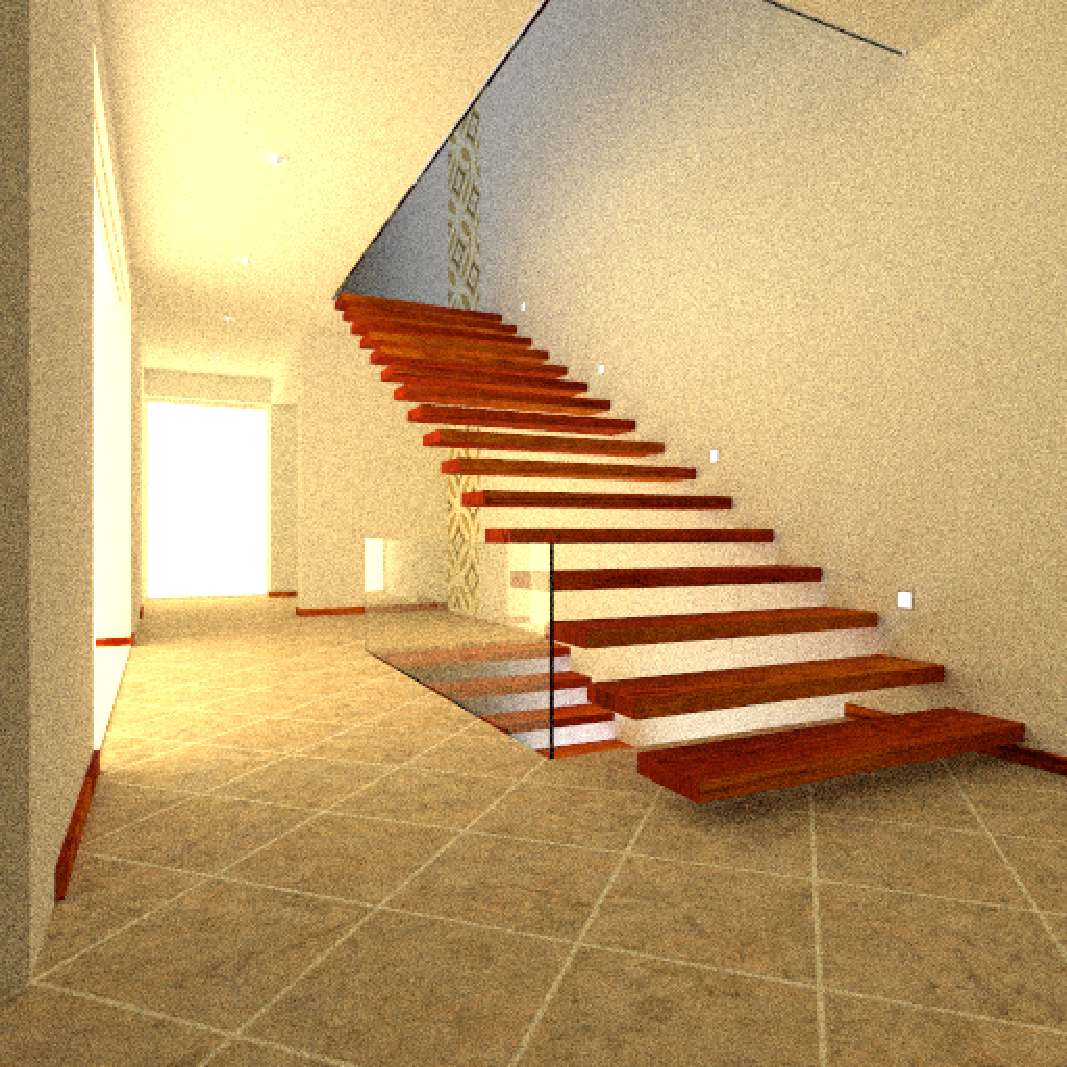
\includegraphics[width=\textwidth]{chapters/chapter_results/correctrender2}
		\caption{Render \texttt{A}}
	\end{subfigure}
	\begin{subfigure}[t]{0.32\linewidth}
		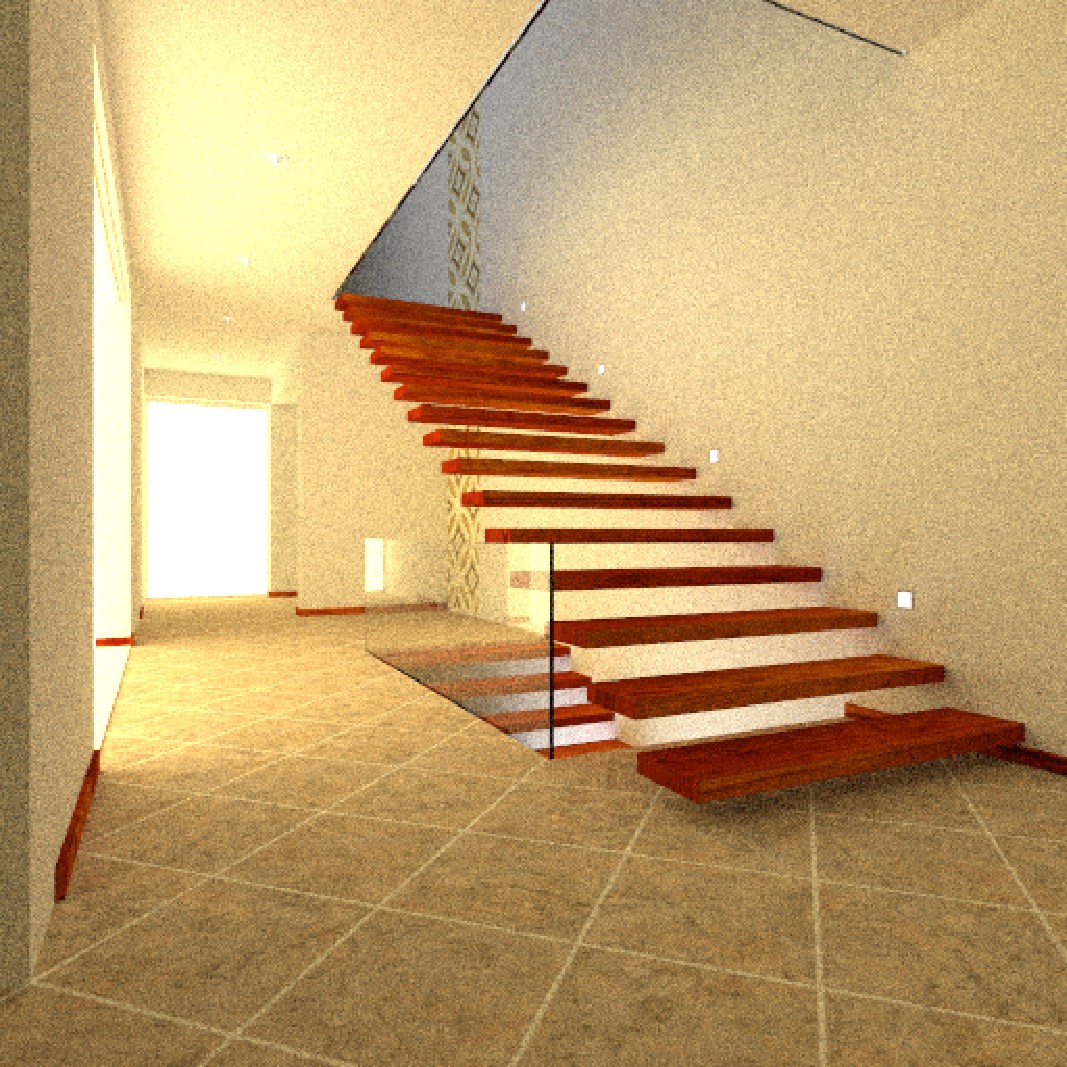
\includegraphics[width=\textwidth]{chapters/chapter_results/wrongrender2}
		\caption{Render \texttt{B}}
	\end{subfigure}
	\begin{subfigure}[t]{0.32\linewidth}
		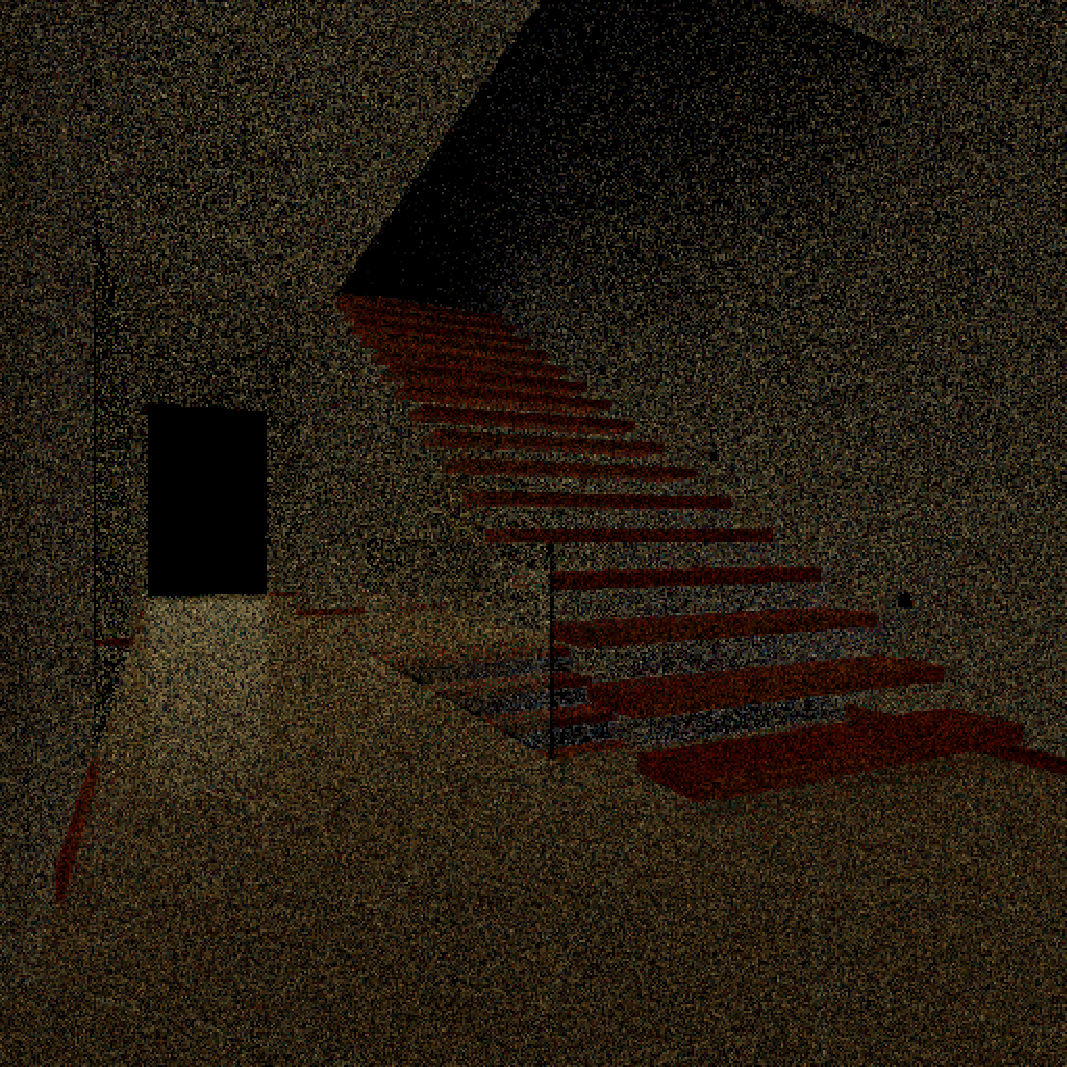
\includegraphics[width=\textwidth]{chapters/chapter_results/render2difference}
		\caption{\texttt{A} $-$ \texttt{B}}
		\label{render2difference}
	\end{subfigure}

	\caption{Render images of the two datasets and their mathematical delta to show their differences.}
	\label{couple2render}
\end{figure}

To provide a more challenging test, the datasets of which renders are shown in figure \ref{couple2render}, both generated by the na\"ive tracer of Yocto/GL \cite{pellacini2019yocto}, have been tinkered to present a very subtle difference. Dataset \texttt{A} is correct while dataset \texttt{B} has been generated after introducing an error in the sampling of microfacet distributions: the direction vector generated according to the distribution has the \textit{y} and \textit{z} components swapped before being transformed from surface space to world space. Logically, this should have generated way more noticeable visual artifacts in the render but, as highlighted by figure \ref{render2difference}, it deceptively looks like there is a miscalculation in the Fresnel term. Without foreseeing this result, an extremely insidious bug has been generated.


\begin{figure}
	\centering
	\begin{subfigure}[t]{0.24\linewidth}
		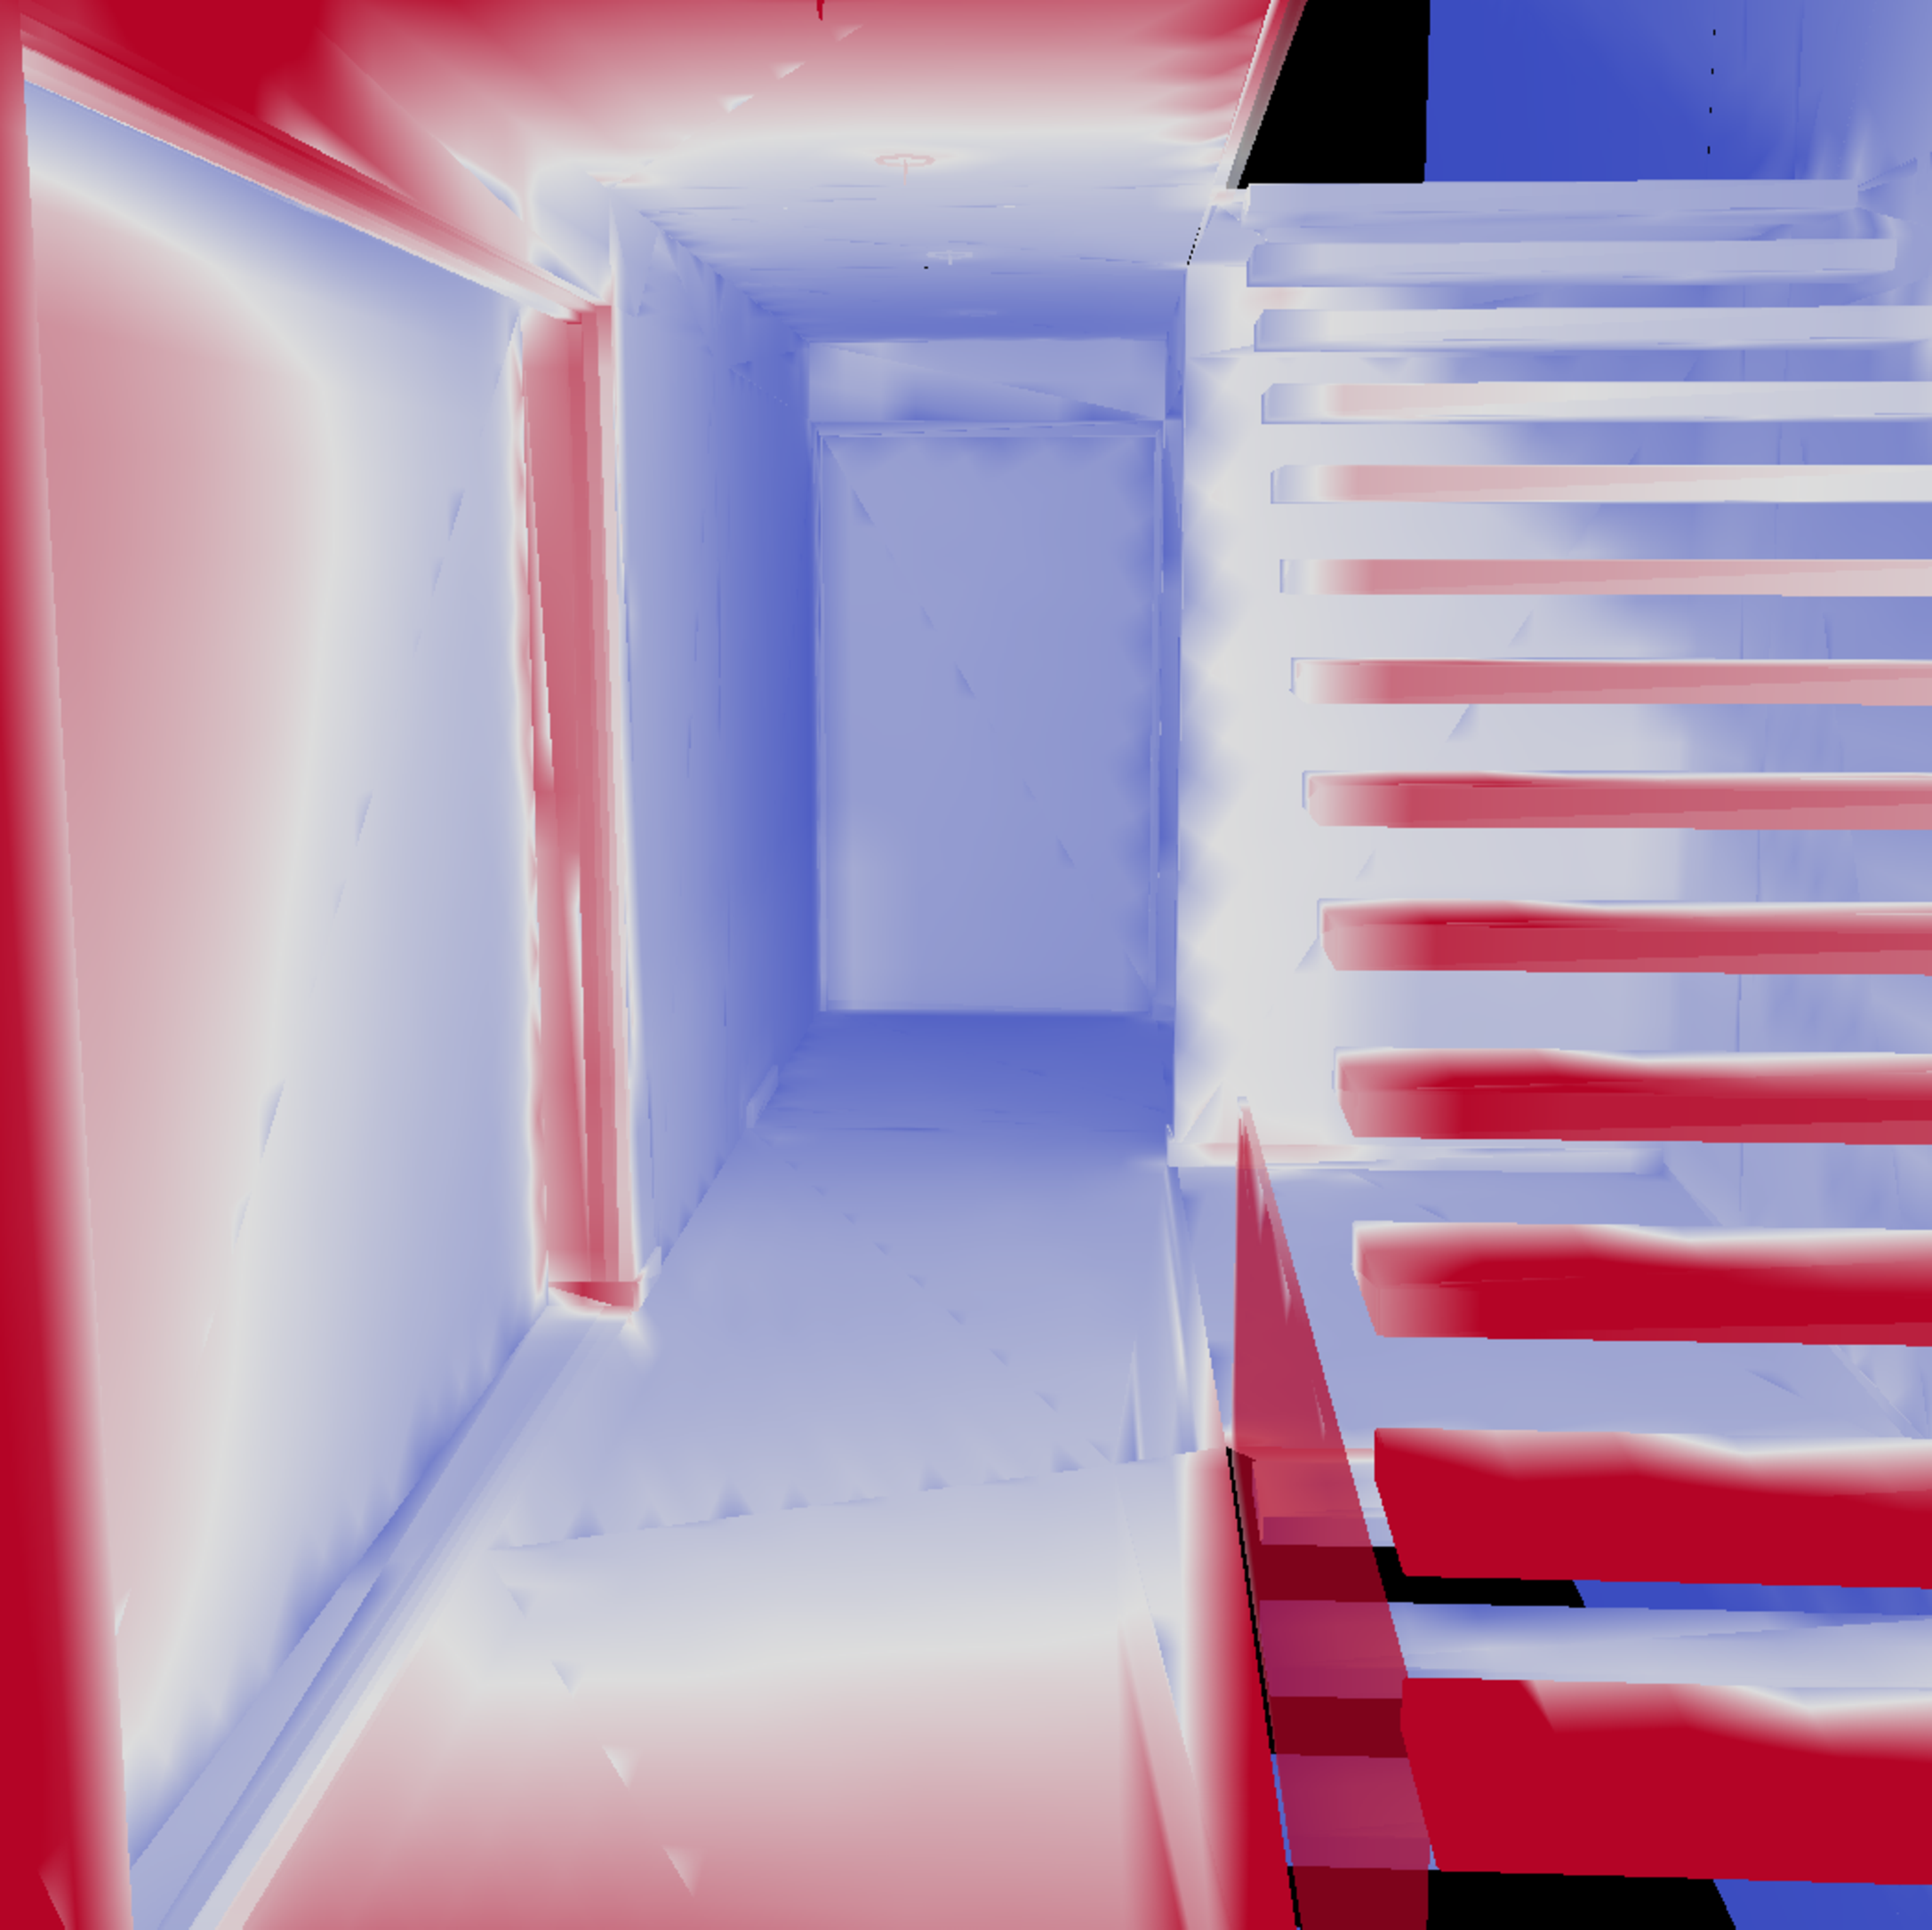
\includegraphics[width=\textwidth]{chapters/chapter_results/correct2heatmap1}
		\caption{Dataset \texttt{A} heatmap 1}
	\end{subfigure}
	\begin{subfigure}[t]{0.24\linewidth}
		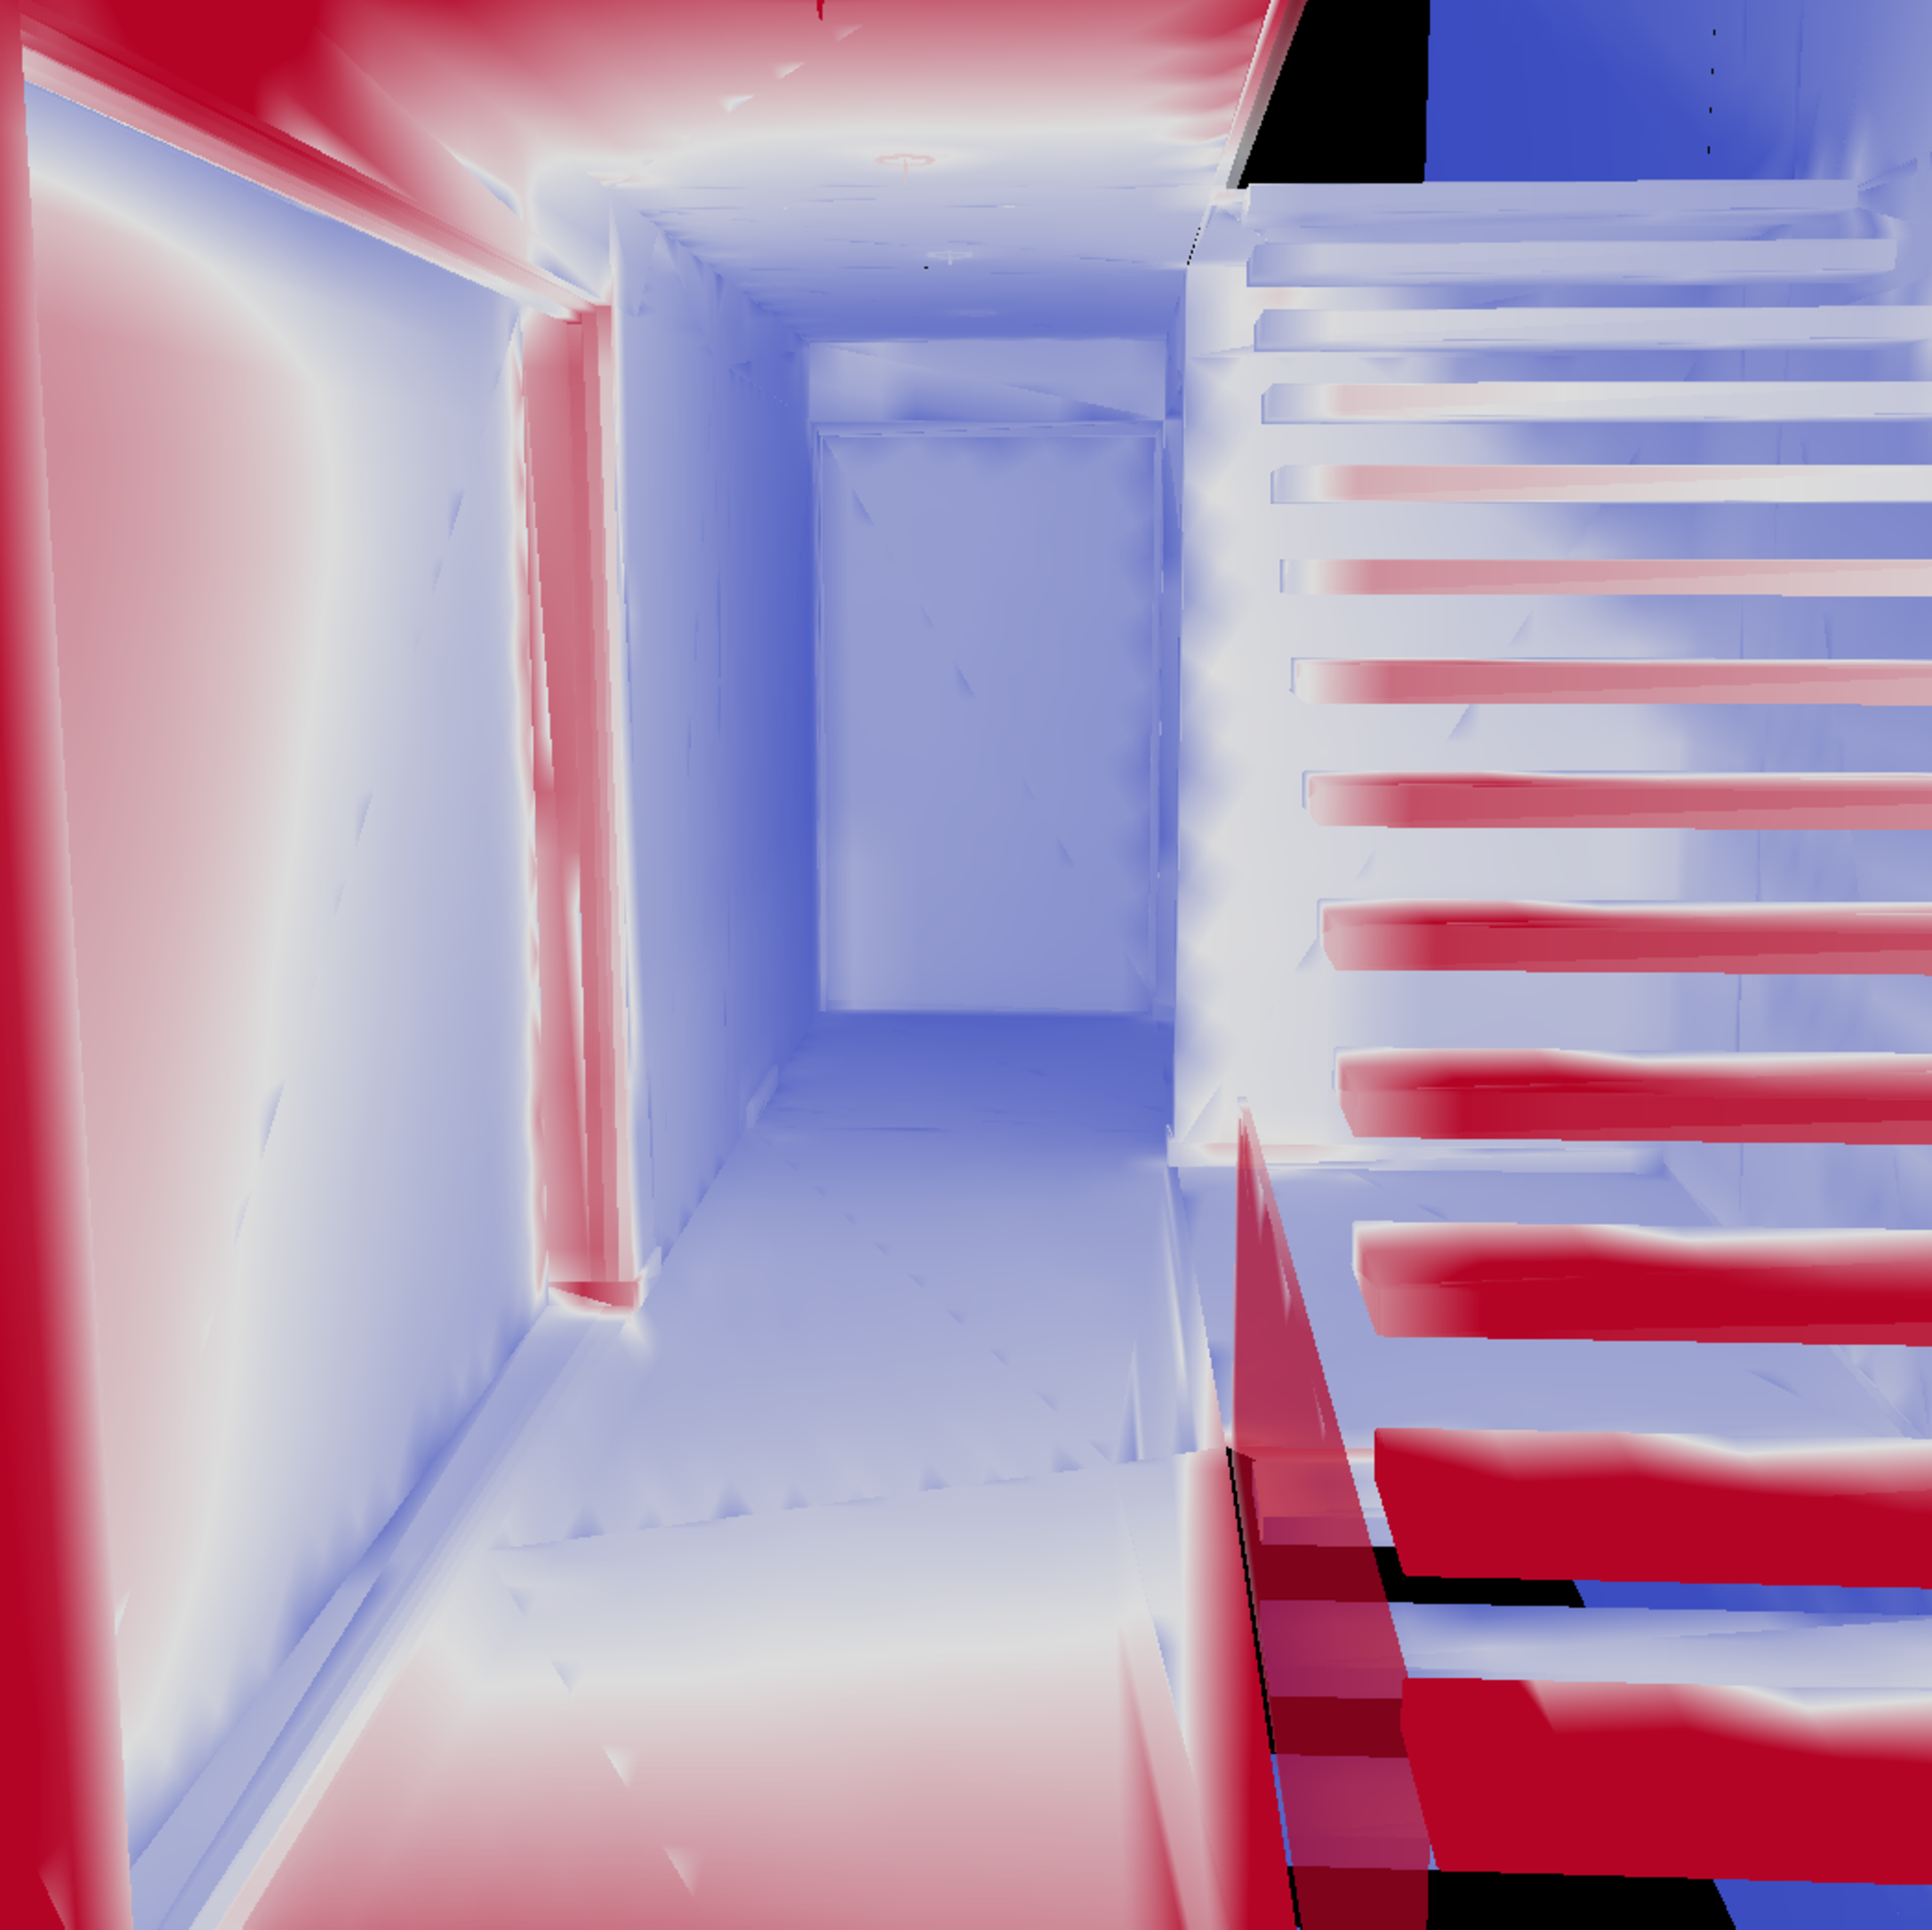
\includegraphics[width=\textwidth]{chapters/chapter_results/wrong2heatmap1}
		\caption{Dataset \texttt{B} heatmap 1}
	\end{subfigure}
	\begin{subfigure}[t]{0.24\linewidth}
		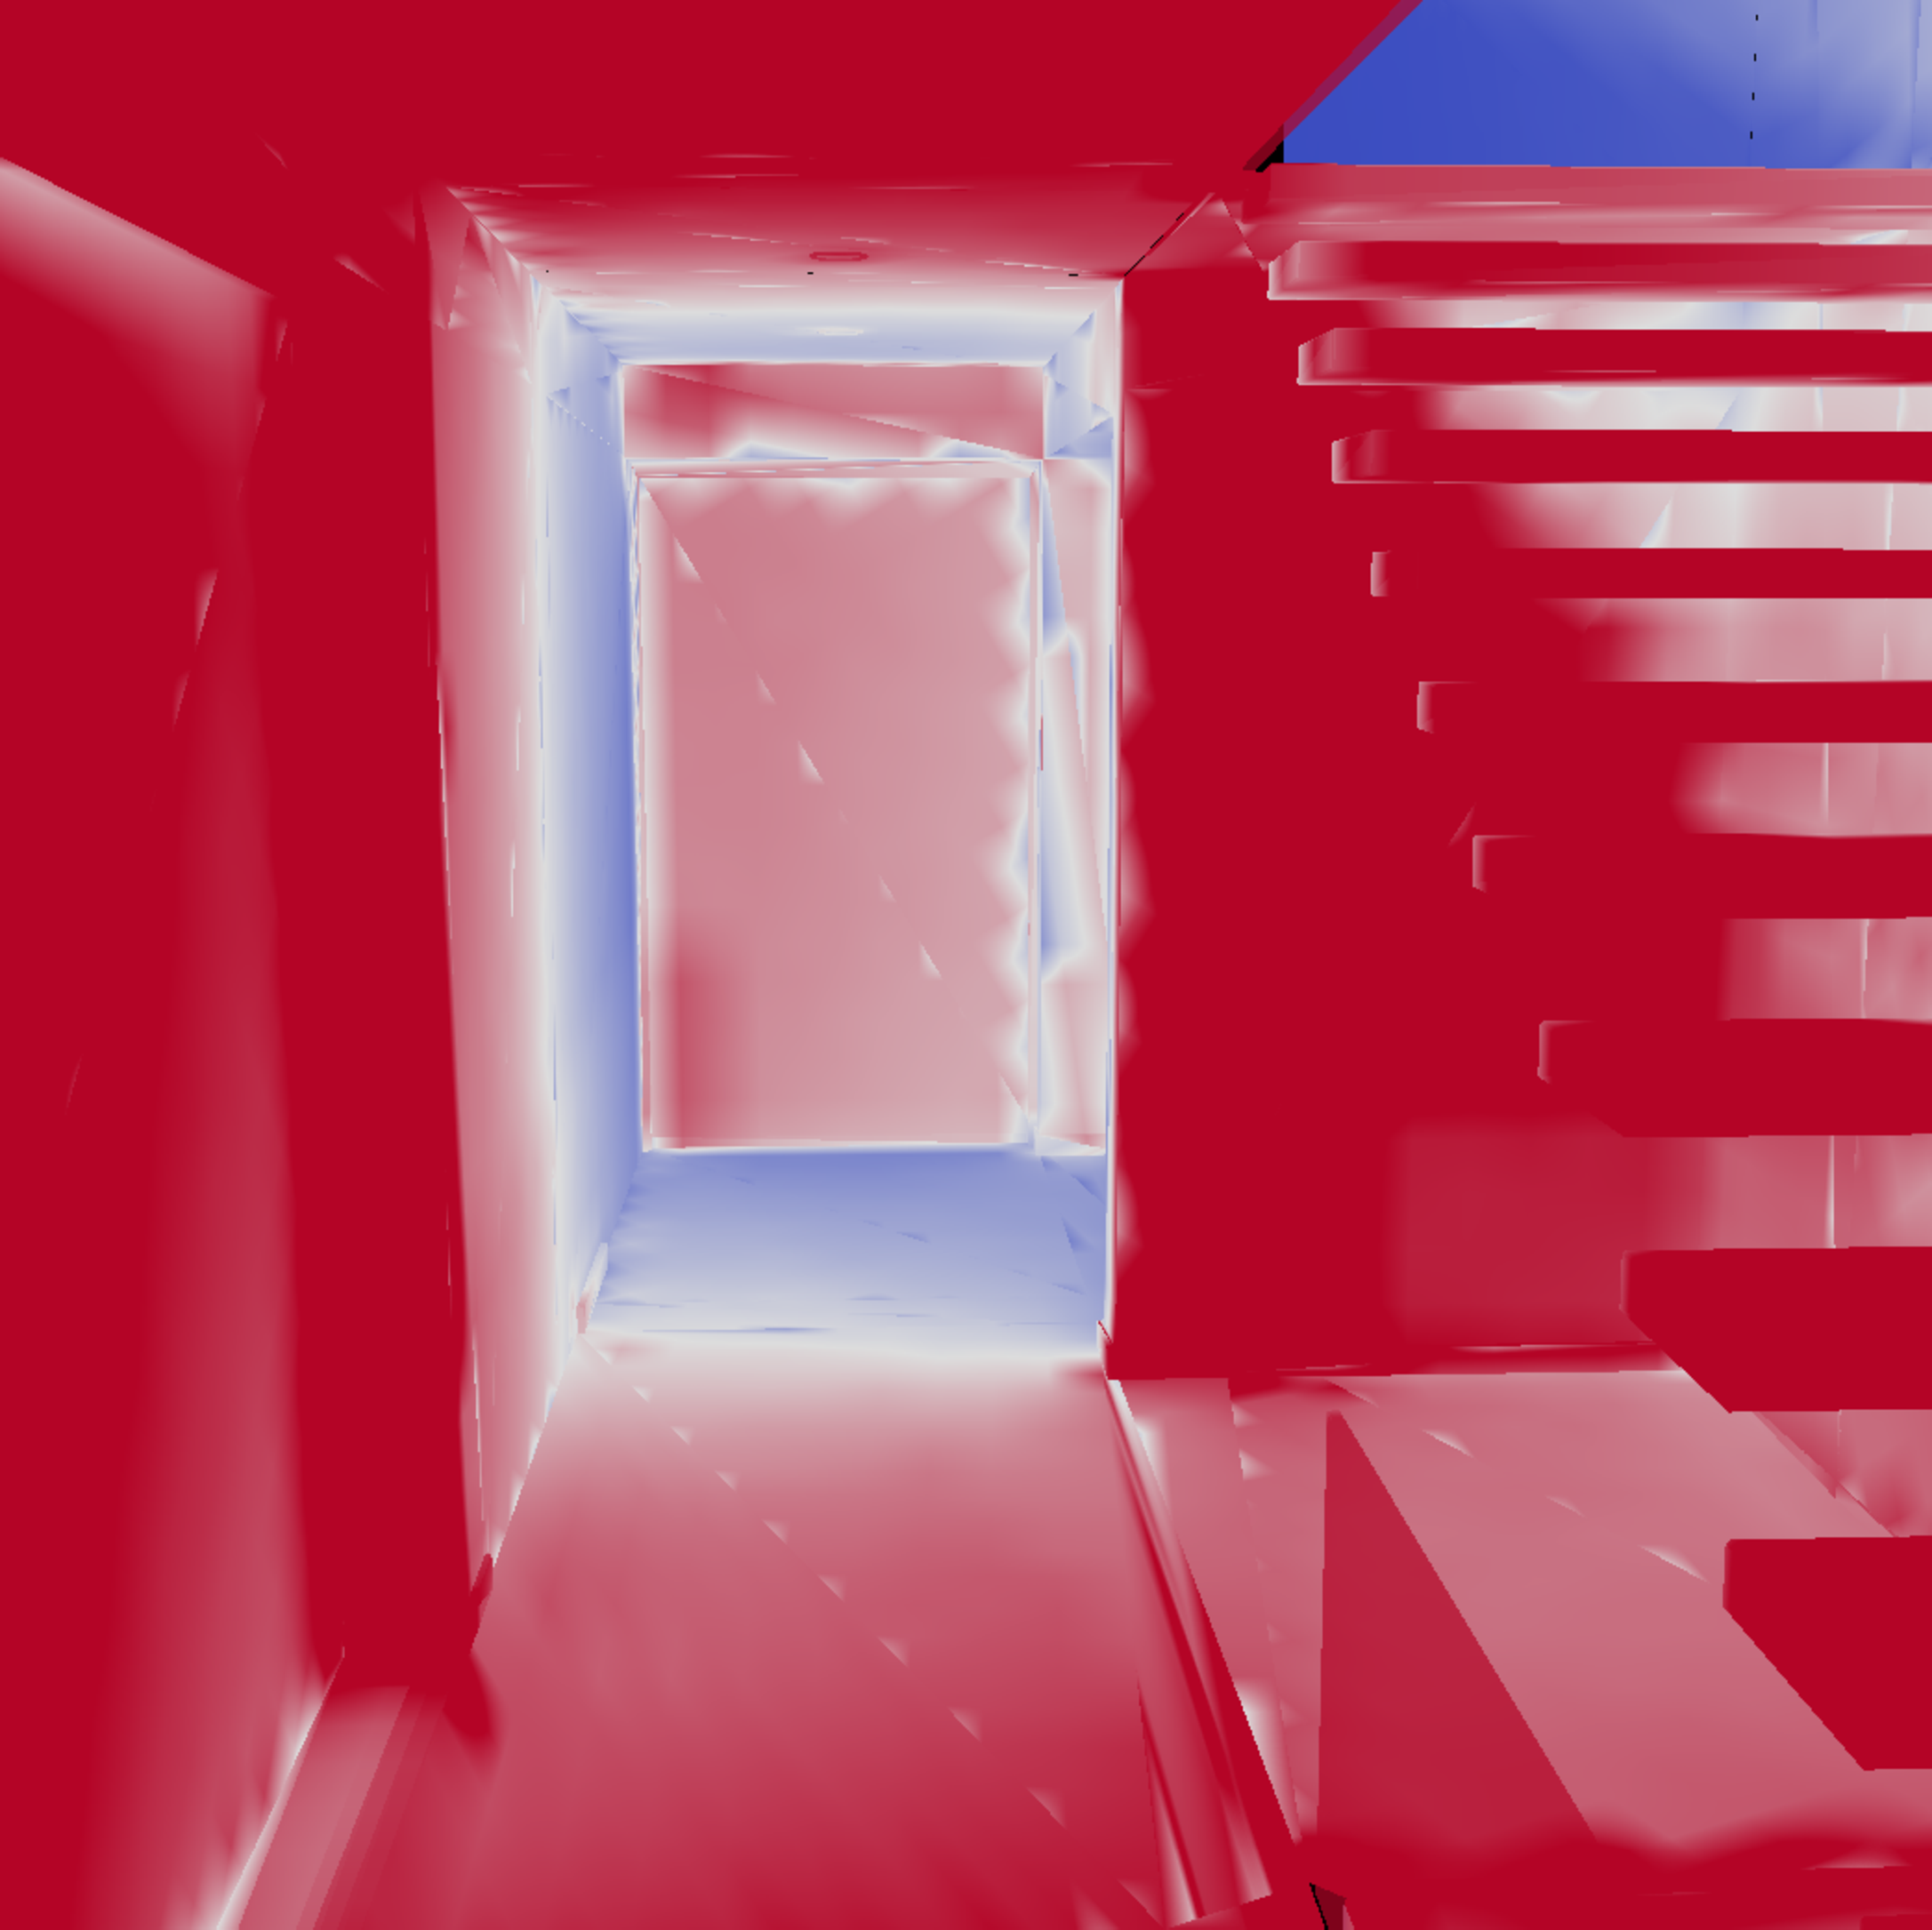
\includegraphics[width=\textwidth]{chapters/chapter_results/correct2heatmap2}
		\caption{Dataset \texttt{A} heatmap 2}
	\end{subfigure}
	\begin{subfigure}[t]{0.24\linewidth}
		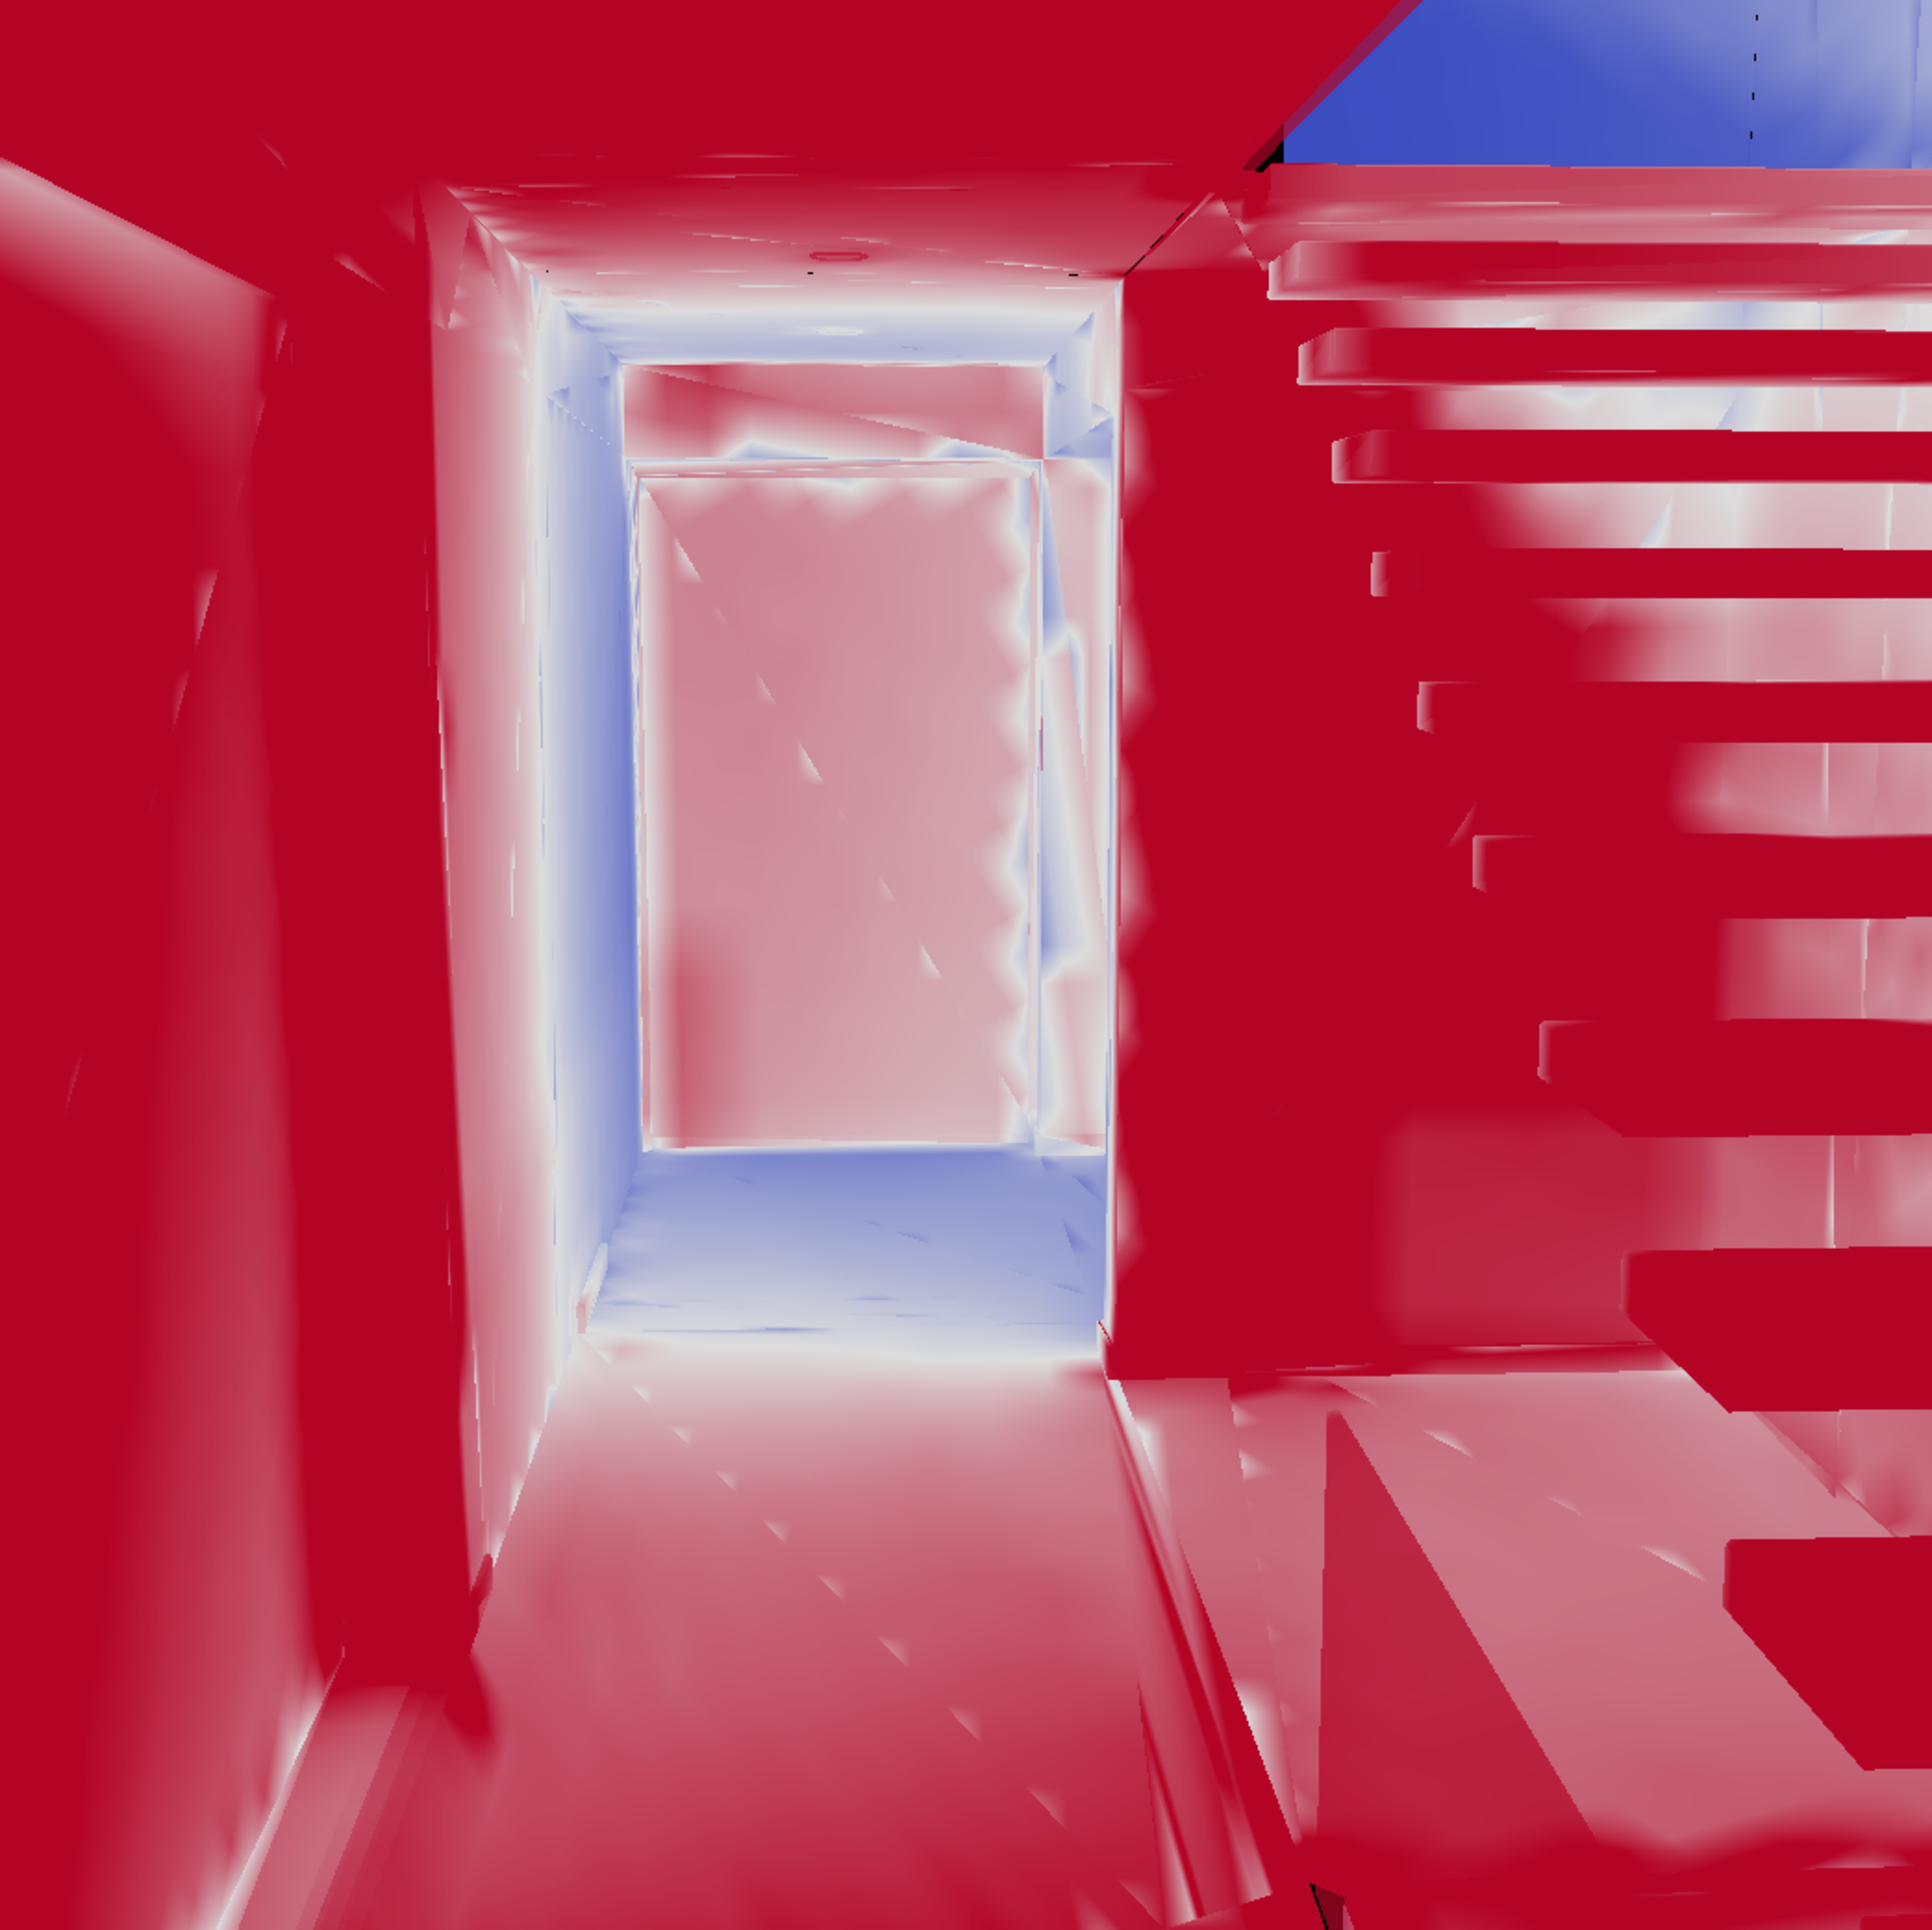
\includegraphics[width=\textwidth]{chapters/chapter_results/wrong2heatmap2}
		\caption{Dataset \texttt{B} heatmap 2}
	\end{subfigure}

	\caption{Heatmap renderings for both datasets from two different cameras and with two different parameters for the \textbf{“Heatmap max”} parameter (for (\textbf{a}) and (\textbf{b}) is set to $100,000$ while for (\textbf{c}) and (\textbf{d}) is set to $40,000$).}
	\label{couple2heatmaps}
\end{figure}

The first instinct was to check the heatmap on the areas where the renders are most different --- that is to say the floor right in front of the light portal at the end of the corridor --- but only minimal differences can be spotted. In the screenshots in figure \ref{couple2heatmaps} vague changes can be seen with a lot of effort, and they just achieve to communicate that the correct dataset --- dataset \texttt{A} --- has a slightly higher bounces density than the wrong dataset. No conclusions can be deducted from this little information.

\begin{figure}
	\centering
	\begin{subfigure}[t]{0.32\linewidth}
		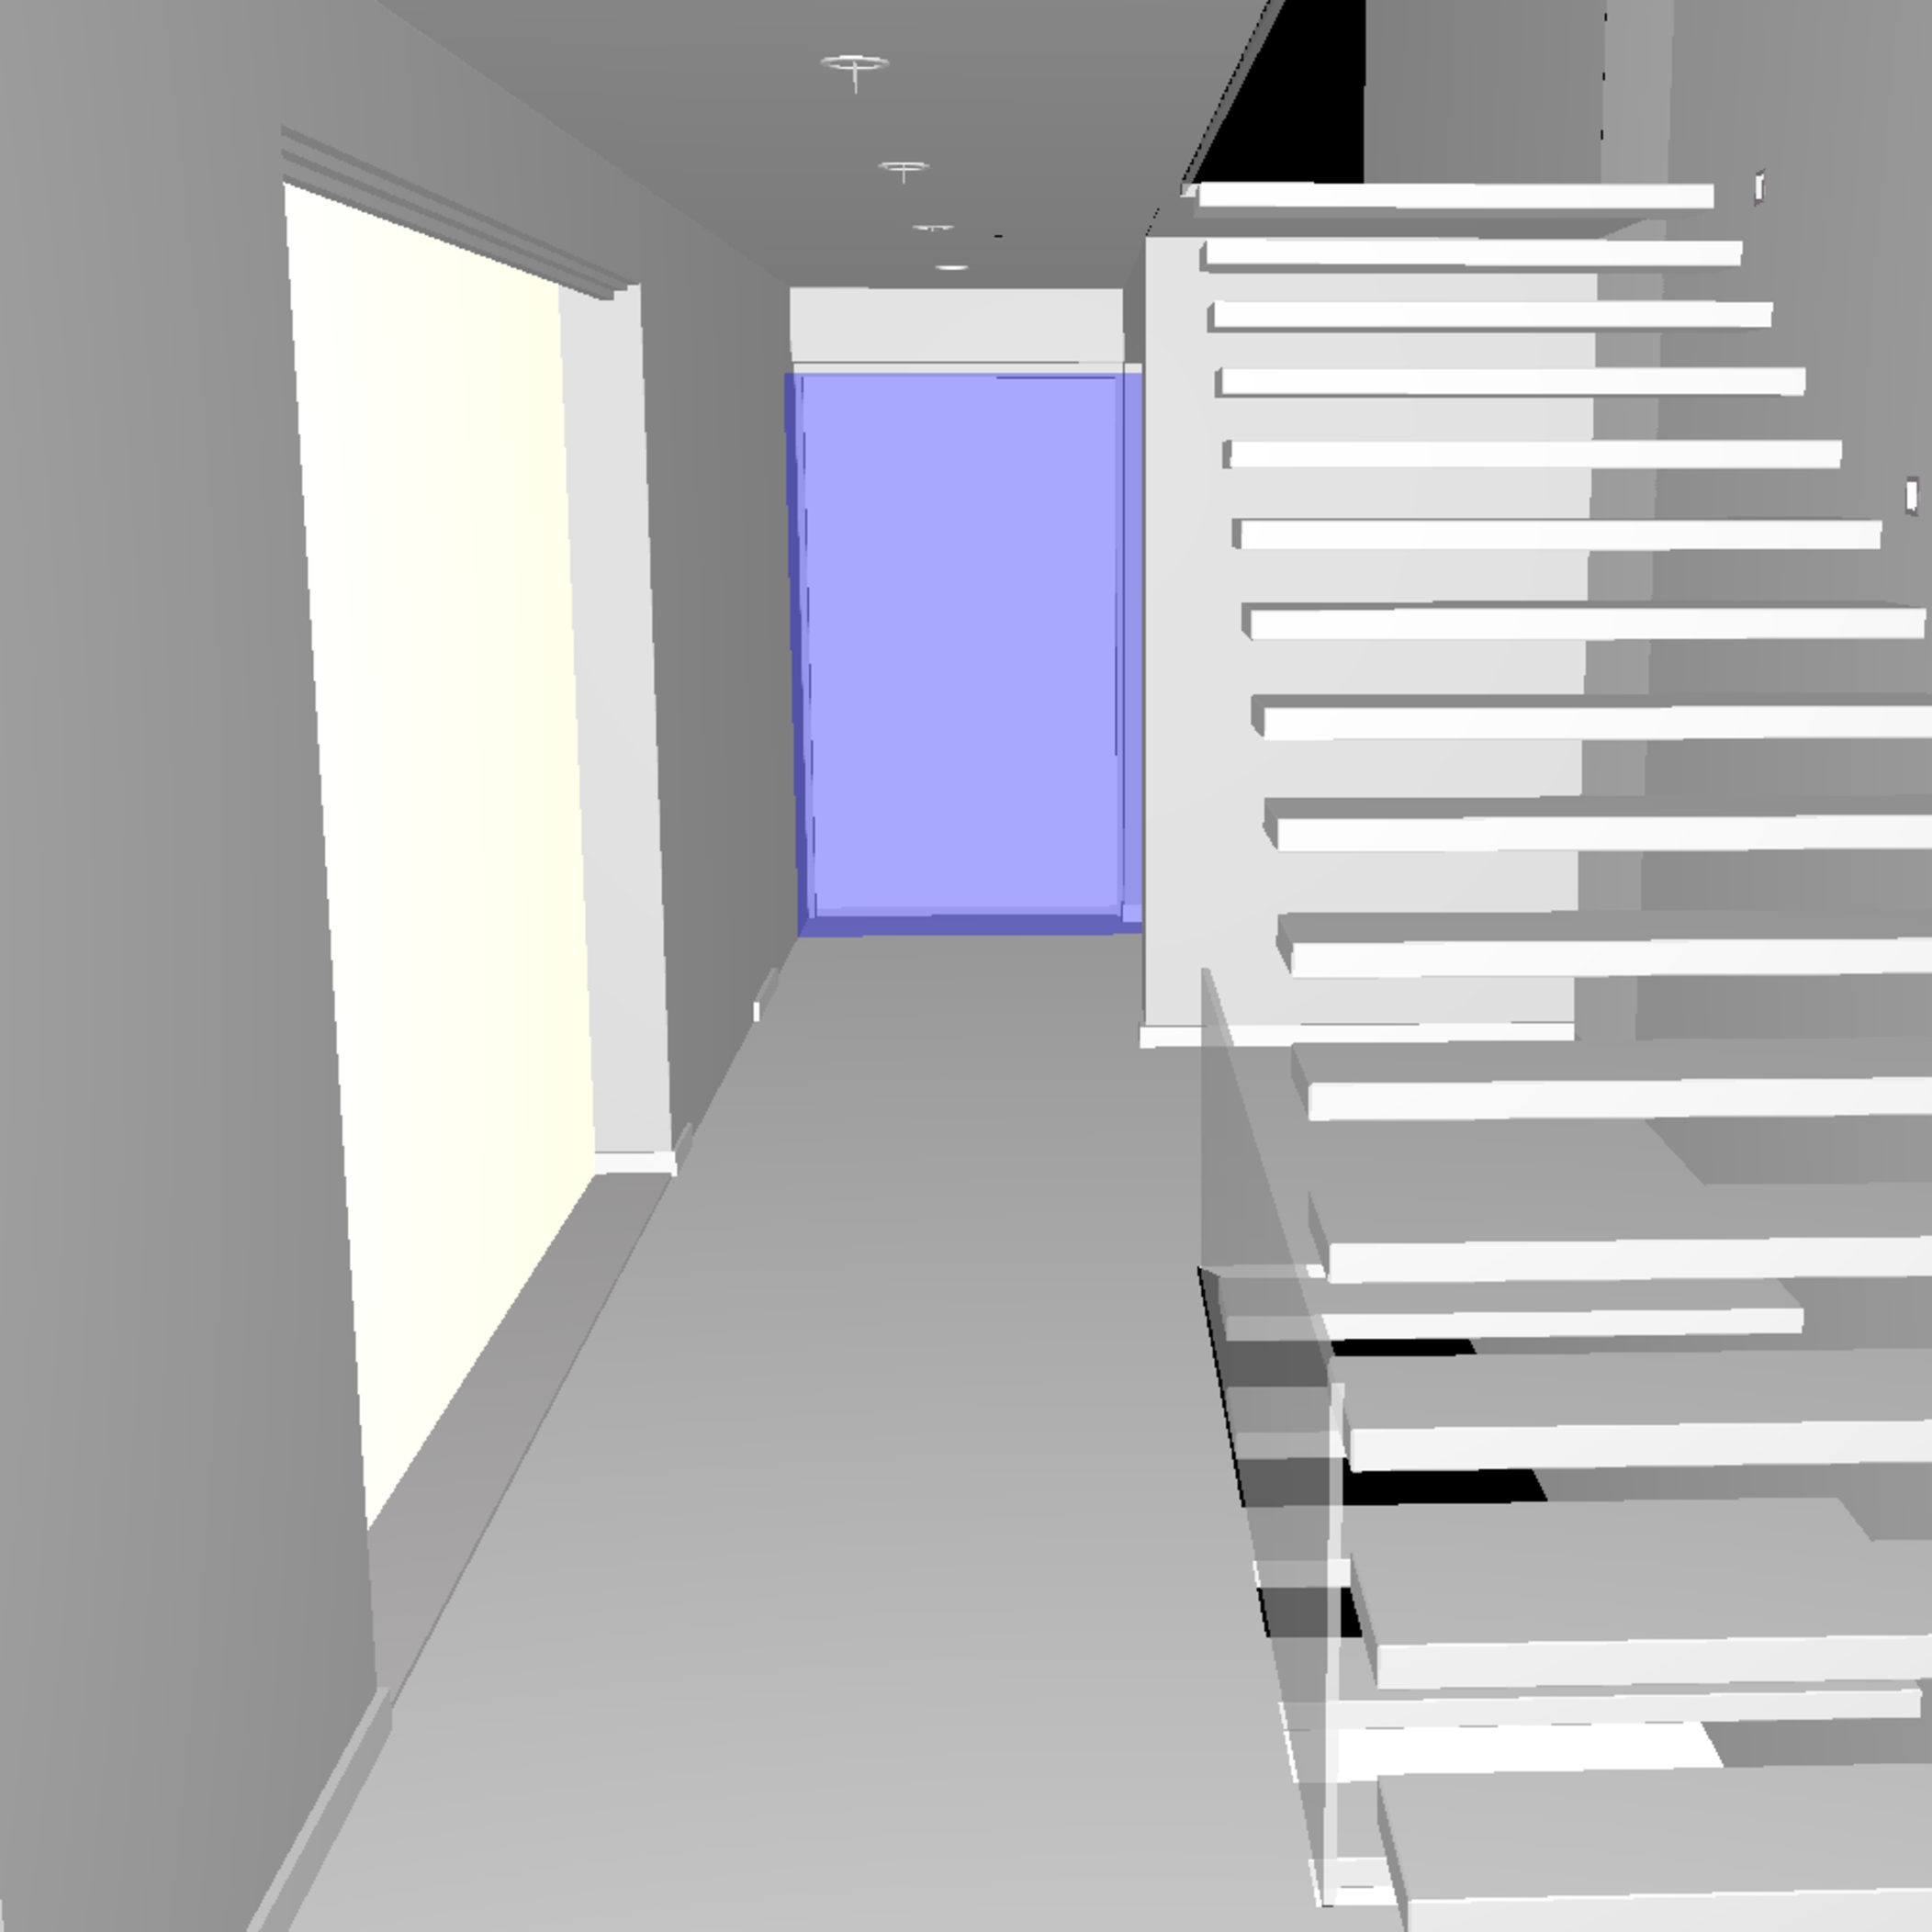
\includegraphics[width=\textwidth]{chapters/chapter_results/ds2filterpos1}
		\caption{Filter position}
	\end{subfigure}
	\begin{subfigure}[t]{0.32\linewidth}
		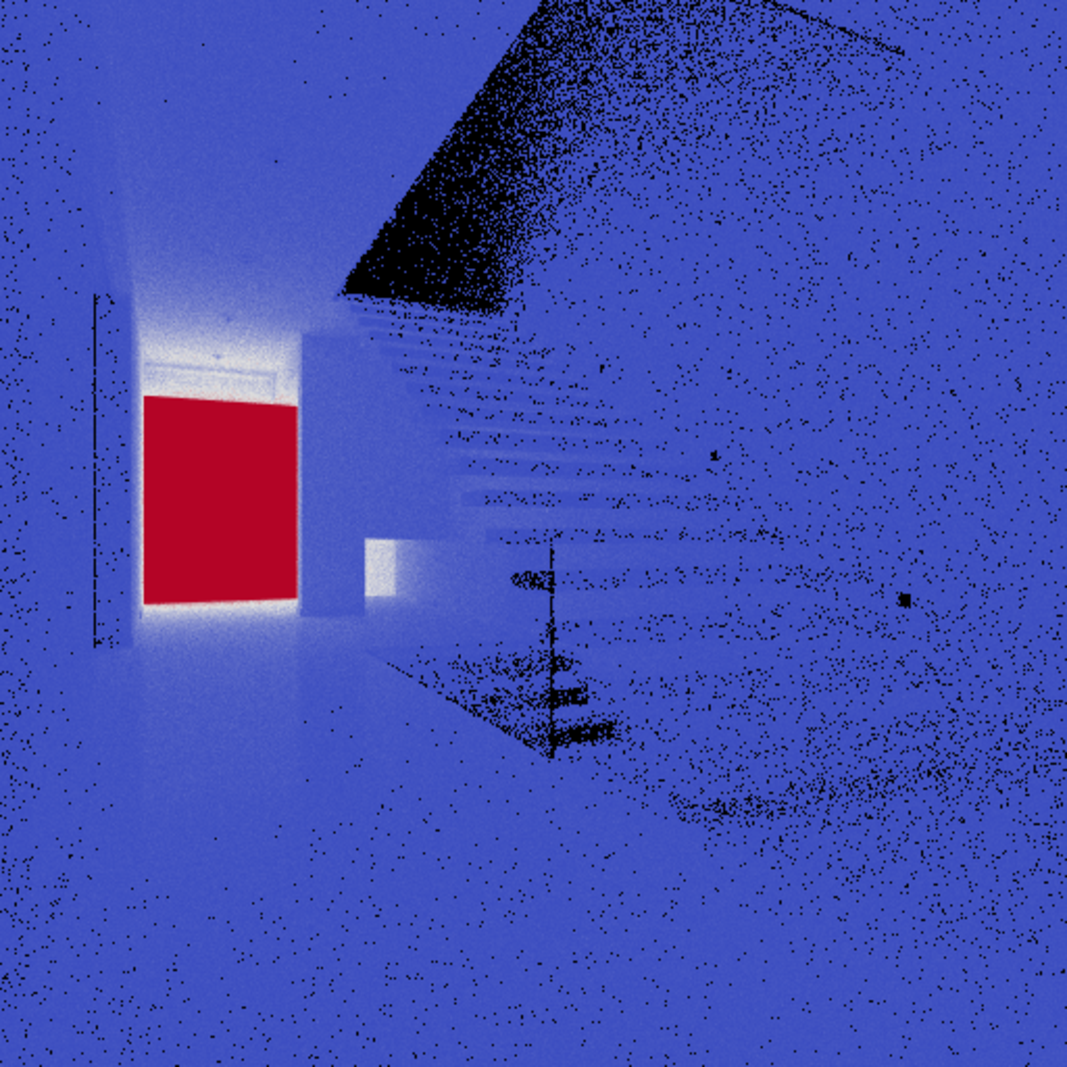
\includegraphics[width=\textwidth]{chapters/chapter_results/correct2ppp}
		\caption{Dataset \texttt{A}}
	\end{subfigure}
	\begin{subfigure}[t]{0.32\linewidth}
		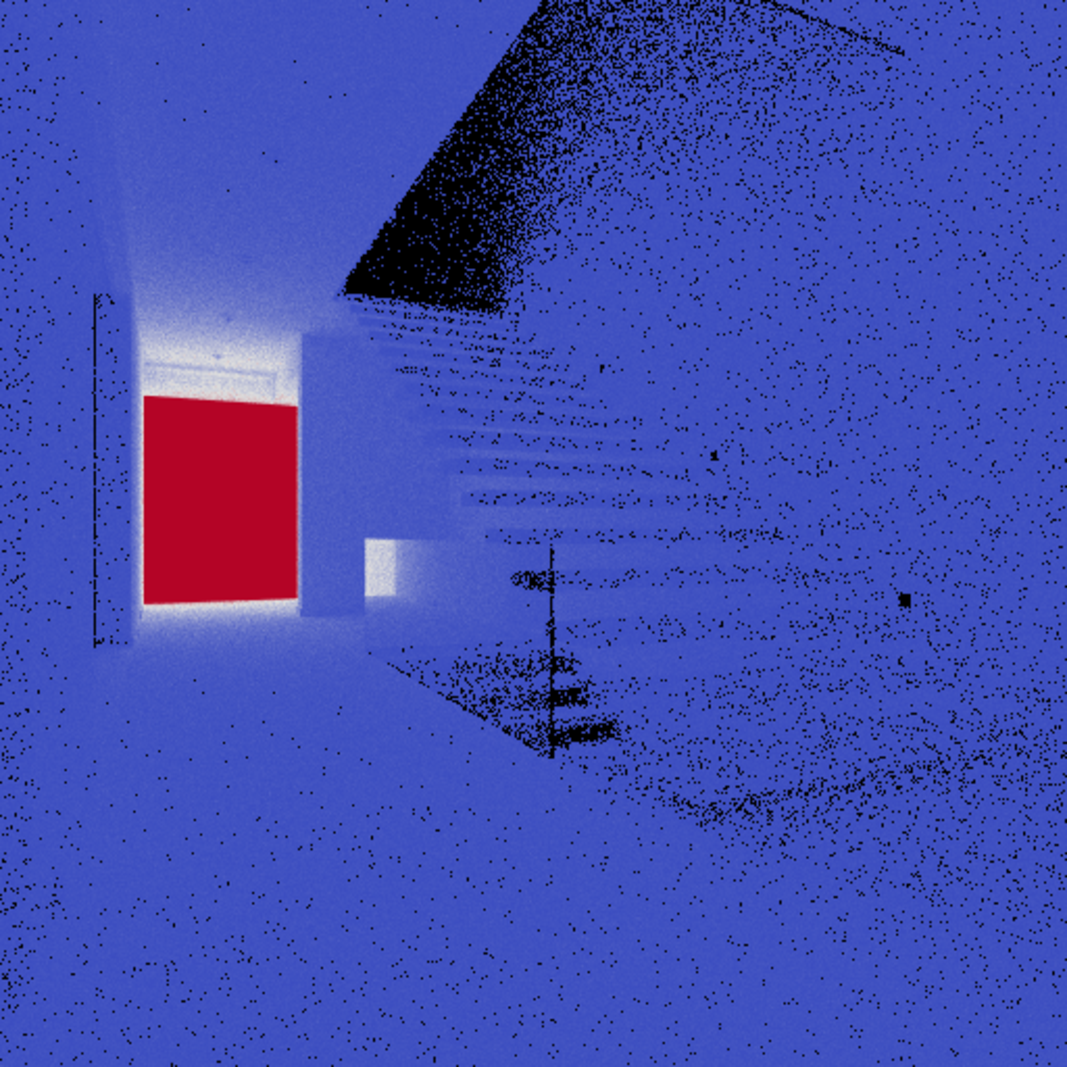
\includegraphics[width=\textwidth]{chapters/chapter_results/wrong2ppp}
		\caption{Dataset \texttt{B}}
	\end{subfigure}

	\caption{Paths per pixel visualization for the window filter shown in (\textbf{a}).}
	\label{couple2ppp}
\end{figure}



